\documentclass[10pt]{article}
\usepackage[utf8]{inputenc}
\usepackage[T1]{fontenc}
\usepackage{amsmath}
\usepackage{amsfonts}
\usepackage{amssymb}
\usepackage[version=4]{mhchem}
\usepackage{stmaryrd}
\usepackage{hyperref}
\hypersetup{colorlinks=true, linkcolor=blue, filecolor=magenta, urlcolor=cyan,}
\urlstyle{same}
\usepackage{graphicx}
\usepackage[export]{adjustbox}
\graphicspath{ {./images/} }
\usepackage{multirow}

\title{gym-hpa: Efficient Auto-Scaling via Reinforcement Learning for Complex Microservice-based Applications in Kubernetes }

\author{José Santos*, Tim Wauters*, Bruno Volckaert*, Filip De Turck*\\
* Ghent University - imec, IDLab, Department of Information Technology\\
Technologiepark-Zwijnaarde 126, 9052 Gent, Belgium\\
Email: josepedro.pereiradossantos @UGent.be}
\date{}


%New command to display footnote whose markers will always be hidden
\let\svthefootnote\thefootnote
\newcommand\blfootnotetext[1]{%
  \let\thefootnote\relax\footnote{#1}%
  \addtocounter{footnote}{-1}%
  \let\thefootnote\svthefootnote%
}

%Overriding the \footnotetext command to hide the marker if its value is `0`
\let\svfootnotetext\footnotetext
\renewcommand\footnotetext[2][?]{%
  \if\relax#1\relax%
    \ifnum\value{footnote}=0\blfootnotetext{#2}\else\svfootnotetext{#2}\fi%
  \else%
    \if?#1\ifnum\value{footnote}=0\blfootnotetext{#2}\else\svfootnotetext{#2}\fi%
    \else\svfootnotetext[#1]{#2}\fi%
  \fi
}

\begin{document}
\maketitle


\begin{abstract}
Containers have revolutionized application deployment and life-cycle management in current cloud platforms. Applications have evolved from large monoliths to complex graphs of loosely-coupled microservices aiming to improve deployment flexibility and operational efficiency. However, modern microservice-based architectures are challenging since proper allocation and scaling of microservices is a difficult task due to their complex inter-dependencies. Existing works do not consider microservice dependencies, which could lead to the application's performance degradation when service demand increases. This paper studies the impact of microservice interdependencies in auto-scaling mechanisms by proposing a novel framework named gym-hpa that enables different auto-scaling goals via Reinforcement Learning (RL). The framework has been developed based on the OpenAI Gym library for the popular Kubernetes (K8s) platform to bridge the gap between RL and auto-scaling research by training RL agents on real cloud environments. The aim is to improve resource usage and reduce the application's response time in future cloud platforms by considering microservice inter-dependencies in horizontal scaling. Experiments with microservice benchmark applications show that RL agents trained with the gym-hpa framework can reduce on average resource usage by $30 \%$ and reduce the application's response time by $25 \%$ compared to default scaling mechanisms.
\end{abstract}

Index Terms-Auto-scaling, Containers, Cloud-native, Microservices, Orchestration, Reinforcement Learning, Kubernetes

\section*{I. Introduction}
Microservice architectures have gradually become the de-facto paradigm for application deployment in modern cloud platforms [1], [2]. The traditional single monolith is decomposed into multiple loosely-coupled microservices, implemented and deployed independently. This paradigm shift improves deployment flexibility and scalability, service portability, and operational efficiency [3]. However, modern microservice-based architectures are challenging to properly orchestrate in current cloud platforms due to their complex microservice inter-dependencies. The increasing adoption of containers calls for efficient deployment and orchestration strategies for microservice applications in current cloud platforms (e.g., Amazon ECS [4], Kubernetes (K8s) [5], Red Hat OpenShift [6]). Also, the next generation of applications, including Extended Reality (XR), Industrial Internet of Things (IIoT), and autonomous vehicles (e.g., cars and Unmanned

Aerial Vehicles (UAVs)) add further complexity and put even more pressure on current cloud infrastructures [7], [8]. The deployment of such applications is hindered by the inability of current infrastructures and protocols to cope with their stringent requirements (e.g., high reliability, low latency, high bandwidth).

Typically, containers support fast adjustments to the application deployment through horizontal and vertical scaling. Horizontal scaling represents the increase (scale-out) or decrease (scale-in) of the number of deployed instances (i.e., containers), while vertical scaling denotes the increase (scale-up) or decrease (scale-down) of the number of resources attributed to each container instance. Service over-provisioning wastes resources and increases costs, while under-provisioning schemes degrade performance and violate Service Level Agreements (SLAs). The goal is to design proper mechanisms capable of scaling resources up and down according to the service demand without human intervention. This procedure is known as Auto-scaling [9], where resources are dynamically added or removed to meet Quality of Service (QoS) requirements. Developing and implementing efficient auto-scaling systems is not a trivial task due to limited hardware resources, dynamic workloads, diverse service requirements, and complex infrastructures. Current literature focuses on either horizontal or vertical elasticity. Fast reactions to small workload variations can be triggered via vertical scaling, while horizontal scaling handles sudden workload peaks. Also, most works mainly address resource utilization in the infrastructure (e.g., CPU and Memory), which is insufficient to satisfy the stringent requirements of microservice applications, especially concerning latency and bandwidth. Existing works (e.g., [10]-[14]) typically scale containers for each microservice separately without considering their microservice inter-dependencies. Most works neglect the impact of these dependencies in large applications on the end-to-end latency and throughput, leading to suboptimal resource usage.

This paper focuses on the impact of microservice interdependencies on auto-scaling mechanisms. The goal is to identify optimal states for each microservice based on the current demand, acknowledging its performance impact in the overall application pipeline. To this purpose, an auto-scaling framework named gym-hpa has been developed to bridge the\\[0pt]
gap between Reinforcement Learning (RL) and auto-scaling research. The framework is inspired on the OpenAI Gym library [15] to train RL agents with different auto-scaling goals on operational cloud environments established with the most popular container orchestration platform, K8s [16]. K8s automates several processes throughout the application lifecycle, including deployment and scaling. Nevertheless, its current auto-scaling policies do not address microservice interdependencies, leading to performance degradation. Also, traditional approaches are mainly focused on threshold-based or Machine Learning (ML)-based methods focused on resource efficiency without any considerations on the application's response time or latency. Our work focuses on horizontal scaling since vertical scaling introduces potentially costly operations. The increase or decrease of container resources could lead to performance degradation or Out of Memory (OOM) errors since containers may no longer fit onto their machines. The main contributions of this paper are:

\begin{itemize}
  \item gym-hpa framework: Implementation of an RL-based framework for proper horizontal scaling of microservicebased applications in K8s clusters. The proposed framework has been open-sourced ${ }^{1}$, allowing researchers to use this framework to evaluate their auto-scaling ideas.
  \item RL implementation: Section V presents the RL design, including observation state, action space, and the reward functions. The approach addresses microservice inter-dependencies and the application's response time, typically overlooked in most works.
  \item Evaluations with microservice benchmarks: The proposed framework has been validated on real-world microservice benchmark applications: a database application named Redis Cluster (RC) [17], and a multi-tier web application named Online Boutique (OB) [18]. Experiments in a K8s cluster show that the presented RL approach can reduce latency on average by $40 \%$ for RC and by $25 \%$ for OB. (Sec. VII).\\
The remainder of the paper is organized as follows: the state-of-the-art on auto-scaling is discussed in the next section. Sec. III discusses application deployment in K8s, describing its terminology. Sec. IV details the gym-hpa framework and Sec. V presents the RL-based auto-scaling approach. Then, Sec. VI describes the evaluation setup, followed by the results in Sec. VII. Sec. VIII concludes this paper.
\end{itemize}

\section*{II. RElated WORK}
Recent surveys [9], [32] address auto-scaling features applied to cloud-based systems. Both works provide a taxonomy of auto-scaling according to several criteria. This section discusses literature across five dimensions: threshold-based, queuing model-based, time series analysis, control theorybased, and ML-based.

Threshold-based techniques [10]-[14] are easy to implement and widely adopted by the industry. Popular orchestration platforms (e.g., K8s, Amazon ECS) rely on best-

\footnotetext{${ }^{1}$ \href{https://github.com/jpedro1992/gym-hpa}{https://github.com/jpedro1992/gym-hpa}
}
effort threshold-based scaling policies based on cluster-level metrics (e.g., CPU usage, the average number of requests). In fact, most cloud providers offer only reactive thresholdbased scaling methods, such as Amazon EC2 [10] and Kubernetes Horizontal Pod Autoscaler (KHPA). Amazon EC2 is particularly well suited for applications with a particular pattern type (e.g., daily or weekly) since rules are specified to handle these traffic patterns. KHPA scales the number of pods based on a certain metric (e.g., CPU usage) by keeping an average of the desired metric by increasing or decreasing the number of deployed pods. The main drawback of these methods is the need for manual tuning to determine appropriate thresholds and scaling actions since, if poorly selected, it significantly impacts the application performance [9]. Vertical scaling techniques [12]-[14] typically resize containers during runtime. Kubernetes Vertical Pod Autoscaler (KVPA) sets container resource limitations by using statistics over a moving window (e.g., for RAM, the 99th percentile over 24 hours). The proposed approach focuses on horizontal scaling since resizing containers may lead to OOM kill or QoS degradation under sudden usage increases. We argue vertical scaling is a risky procedure needing further research to prove container resources adapted at runtime do not compromise performance.

Queuing model-based methods are popular for analyzing Internet applications. These techniques estimate the performance metrics and the waiting time for the requests. Recent works have applied queuing theory to auto-scaling [19], [20]. These methods focus mainly on reducing costs while maintaining the application's Service Level Objectives (SLOs). All queuing-based methods are applicable for multi-tier applications, however, they mainly rely on stationary systems where the demand does not change over time. These models depend on known parameters (e.g., the arrival rate of service requests), meaning that model and metrics recalculation is needed for dynamic workloads.

Time series analysis usually involves a two-step process: workload forecasting is applied, and then scaling actions are triggered based on the predicted workload. Nevertheless, most methods [21]-[23] rely on predefined thresholds since actions are triggered if the predicted metric goes beyond a certain threshold. Workload prediction models are typically applied to perform adequate scaling actions, leading to resource efficiency and minimal QoS impact [21]. However, the applicability of these methods to all types of workloads is difficult, and can take a significant amount of time to predict incoming requests [22] or the subsequent resource consumption. These often also consider a single microservice. In contrast, the proposed approach finds appropriate scaling actions depending on the current status of multiple microservices.

Control theory-based methods [24]-[27] typically consist of two phases (i.e., analysis and planning) coming from the Monitoring, Analysis, Planning and Execution (MAPE) loop [33]. The system behavior is modified based on the output and reference values. The goal is to adjust the output to the reference values based on feedback from the system. In auto-scaling, the desired SLA is the reference value, and the

TABLE I: Comparison among different auto-scaling methods.

\begin{center}
\begin{tabular}{|c|c|c|c|c|c|c|c|}
\hline
Existing Work & Dimension & Type & Policy & Virtualization & Metrics & Microservice Dependencies & Evaluation Method \\
\hline
Amazon EC2 [10] & T & H & R & VMs + C & e.g., CPU, RAM & $\times$ & A \\
\hline
KHPA [11] & T & H & R & C & e.g., CPU, RAM & $\times$ & K \\
\hline
KVPA [12] & T & V & R & C & e.g., CPU, RAM & $\times$ & K \\
\hline
Al-Dhuraibi, Y., et al. [13] & T & V & R & C & CPU + RAM & $\times$ & D \\
\hline
Rattihalli, G., et al. [14] & T & V & R & C & CPU + RAM & $\times$ & A + K \\
\hline
Gergin, I., et al. [19] & Q & H & R & VMs & RT & $\times$ & A \\
\hline
Danilo, A., et al. [20] & Q & H & R & VMs & CPU + RT & $\times$ & S + T \\
\hline
Calheiros, R. N., et al. [21] & TS & H & P & VMs & e.g, CPU, RT & $\times$ & S \\
\hline
Messias, V. R., et al. [22] & TS & H & $\mathrm{R}+\mathrm{P}$ & VMs & RT & $\times$ & S \\
\hline
Kumar, J., et al. [23] & TS & H & $\mathrm{R}+\mathrm{P}$ & VMs & R & $\times$ & S \\
\hline
Baresi, L., et al. [24] & CT & H & R & VMs + C & e.g., CPU & $\times$ & A \\
\hline
Farokhi, S., et al. [25] & CT & V & R & VMs & e.g., RAM, RT & $\times$ & T \\
\hline
Nouri, S. M. R.,, et al. [26] & CT + ML & H & R & VMs & e.g., CPU, RT & $\times$ & T \\
\hline
Toosi, A. N., et al. [27] & CT & H + V & R & VMs & e.g., CPU, TL & $\checkmark$ & S \\
\hline
Rossi, F., et al. [28] & ML & H + V & $\mathrm{R}+\mathrm{P}$ & C & e.g., CPU, RAM & $\times$ & S + D \\
\hline
Lee, D., et al. [29] & ML & H & P & VMs & T + RT & $\checkmark$ & O \\
\hline
Rzadca, K., et al. [30] & ML + TS & H + V & P & C & e.g., CPU, RAM & $\times$ & T \\
\hline
Toka, L., et al. [31] & ML + TS & H & $\mathrm{R}+\mathrm{P}$ & C & CPU + R & $\times$ & K \\
\hline
Our work & T + ML & H & $\mathrm{R}+\mathrm{P}$ & C & e.g. RT, CPU, RAM & $\checkmark$ & S + K \\
\hline
\end{tabular}
\end{center}

Dimension: $\mathrm{T}=$ Threshold-based, $\mathrm{Q}=$ Queuing model-based, $\mathrm{TS}=$ Time Series analysis, $\mathrm{CT}=$ Control theory-based, ML = ML-based.\\
Type: $\mathrm{H}=$ Horizontal, $\mathrm{V}=$ Vertical.\\
Policy: $\mathrm{R}=$ Reactive, $\mathrm{P}=$ Proactive.\\
Virtualization: VMs = Virtual Machines, $\mathrm{C}=$ Containers.\\
Metrics: CPU = CPU usage, RAM = Memory usage, $\mathrm{T}=$ Throughput, $\mathrm{RT}=$ Response time, $\mathrm{TL}=$ Traffic load, $\mathrm{R}=$ Number of requests per second. Microservice Dependencies: $\checkmark=$ addressed, $X=$ not considered.\\
Evaluation Method: A = Amazon AWS, $\mathrm{K}=$ Kubernetes, $\mathrm{D}=$ Docker, $\mathrm{O}=$ Openstack, $\mathrm{S}=$ Simulation, $\mathrm{T}=$ Testbed.\\[0pt]
output consists of performance metrics (e.g., CPU usage). Experiments show that these approaches significantly reduce deployment costs by improving overall memory utilization [25] and by mitigating SLA violations [27]. However, these techniques are highly dependent on the controller design and the target application. Their main drawback occurs when dealing with dynamic and unpredictable workloads. Several works tackle these issues by combining control-theory methods with ML-based techniques or even time series analysis to predict future demands inside the controller and adapt resources accordingly. Their main advantage is the reduced execution time and high efficiency in the scaling process.

ML-based techniques [28]-[31] are popular nowadays. These methods aim to build a model for resource estimation under a specific workload. These approaches are robust to dynamic demands since the algorithm adjusts the model parameters if any notable event occurs (i.e., online learning). The model also can be trained offline, but it would often require significant human intervention, losing the main benefit of these algorithms. Google Autopilot has been presented in [30]. It automatically configures resources, adjusting the number of concurrent tasks in a job (i.e., horizontal scaling) and the CPU/RAM limits for individual tasks (i.e., vertical scaling). Autopilot aims to reduce the difference between resource limits and actual resource usage while minimizing the risk of OOM errors and performance degradation due to CPU throttling. Autopilot applies ML algorithms to historical data to learn patterns from previous task executions. Results show that Autopilot significantly reduces resource utilization and minimizes OOM errors. The main drawback of ML-based\\
approaches is the high execution time to converge to a stable model and thus causes auto-scaling to perform poorly during the learning period.

Table I shows a comparison of all methods introduced in this section. All works have been classified based on their main characteristics. However, the quantitative assessment is challenging since these methods are designed for a particular system or virtualization technology. To the best of our knowledge, no standard testing framework for auto-scaling features exists. Previously, we have proposed scheduling extensions for the K8s platform [34] [35] addressing microservice-based chaining concepts. This paper extends our previous work by focusing on the other important aspect of the life cycle management of containerized applications: auto-scaling. The paper introduces the gym-hpa framework bridging the gap between RL and auto-scaling research. RL algorithms train on real cloud environments based on the K8s platform. The work differs from the current literature by addressing microservice inter-dependencies and the application's response time as an auto-scaling objective. The proposed gym-hpa allows researchers to validate their different auto-scaling ideas on a real cloud environment.

\section*{III. APPLICATION DEPloymENT IN KubERNETES (K8S)}
With the massive adoption of microservice patterns and containers, several orchestration platforms have been developed by the Industry and open-source communities. K8s is the most popular today, providing several software components for the automatic life cycle management of containerized applications across a set of cluster nodes. K8s follows the known master-slave model, where at least one master node\\
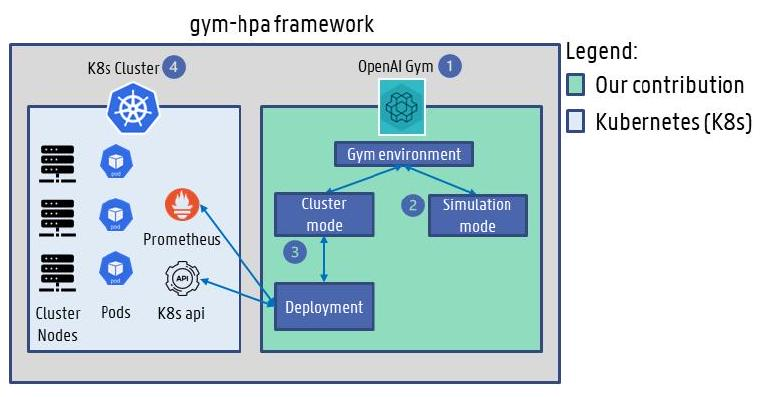
\includegraphics[max width=\textwidth, center]{2024_11_17_21ad14b6196e5740bf69g-4}

Fig. 1: Illustration of the gym-hpa framework.\\
manages containers across multiple worker nodes (slaves). Master nodes typically have more computing power to operate all software components (e.g., API server, Kubelet, Controller Manager) responsible for handling the complete life cycle workflow of containerized applications.

Microservices in K8s are often tightly coupled into a group of containers named a pod, the smallest working unit in K8s. A pod represents the collection of containers and volumes (storage) running in the same execution environment [5]. K8s establishes a connection of identical pods via a Deployment [36], but it does not natively support the aggregation of different pods into a particular application. Developers need to set up individual KHPA components to each deployment to handle horizontal scaling across their entire application. Thus, KHPA currently handles horizontal scaling for each deployment without any knowledge about the microservice interdependencies of those pods. The next section describes the gym-hpa framework that considers microservice dependencies by combining several K8s deployments into an application.

\section*{IV. THE GYM-HPA FRAMEWORK: SYSTEM ARCHITECTURE}
\section*{A. System Overview}
Fig. 1 shows an overview of the gym-hpa framework and its main software components. One of the main building blocks is the OpenAI Gym module (1), where different gym environments are available for RL training. Two evaluation modes are supported by gym-hpa: simulation (2) and cluster. The simulation mode corresponds to a discrete-event simulator to reenact the behavior of multiple service requests for a given application deployed on the K8s platform. The application's resource usage (e.g., CPU and Memory usage) and the number of deployed pods is updated during the simulation based on scaling actions and the current service demand. Sec. VI-B shows how datasets were created for the simulation mode based on the evaluated applications to create near-real experiments. In contrast, the cluster mode corresponds to RL training on a real cluster environment through the Deployment component (3). This component interacts with a K8s cluster (4) via the K8s Application Programming Interface (API) to retrieve information about the given application and via the Prometheus API [37], a well-known monitoring platform, to retrieve its current usage metrics. Further explanations are

TABLE II: Deployment status in the gym-hpa framework.

\begin{center}
\begin{tabular}{|c|l|}
\hline
Symbol & Description \\
\hline
$A$ & The application $a$. Each application consists of a set of \\
$D_{a}$ & Therent deployments $d \varepsilon D_{a}$. \\
$N_{a}$ & The set of deployments belonging to the application $a$. \\
$C_{d}$ & The set of container names $c \varepsilon C$ for deployment $d$. \\
$I_{d}$ & The set of container images $i \varepsilon I$ for deployment $d$. \\
$P_{d}$ & The set of all pods belonging to the deployment $d \varepsilon D$. \\
$\alpha_{d, m a x}$ & The maximum replication allowed for deployment $d$. \\
$\alpha_{d, m i n}$ & The minimum replication allowed for deployment $d$. \\
 & The request vector of deployment $d . r$ denotes resources as \\
$\gamma_{d,[r]}$ & CPU (in m) and memory (in Mi). m stands for millicore and \\
 & Mi stands for mebibyte. \\
$\Gamma_{d,[r]}$ & The limit vector of deployment $d . r$ denotes resources as CPU \\
 & (in m) and memory (in Mi). \\
$\rho_{d,[r]}$ & The total usage vector of deployment $d . r$ denotes resources \\
$\sigma_{d, i}$ & as CPU (in m) and memory (in Mi). \\
$\sigma_{d, o}$ & The total traffic received (in Kbps) of deployment $d$. \\
$R_{d}$ & The current number of deployed pods for deployment $d$. \\
$T$ & The threshold for resource usage. Default: 0.75. \\
$\Omega_{c}$ & The CPU weight for replica calculation. Default: 0.7. \\
$\Omega_{m}$ & The memory weight for replica calculation. Default: 0.3. \\
$\lambda_{[r]}$ & The target resource usage vector. $r$ denotes resources as CPU \\
$\omega_{d}$ & (in m) and memory (in Mi). \\
$\tau_{a}$ & The desired number of replicas (i.e., pods) for deployment $d$. \\
$\Psi_{a}$ & The application latency (in ms). \\
 &  \\
\end{tabular}
\end{center}

given below on how the Deployment component and K8s interact.

\section*{B. Kubernetes Integration}
Table II shows the available information in the Deployment component based on a K8s deployment. The framework allows developers to specify the microservices $\left(D_{a}\right)$ belonging to an application (a). Input information (e.g., $P_{d}, N_{a}$ ) is retrieved from the K8s API, while its current status (e.g., $R_{d}, \rho_{d,[r]}$ ) is retrieved from the Prometheus API. An important concept in K8s is resource requests $\left(\gamma_{d,[r]}\right)$ and limitations $\left(\Gamma_{d,[r]}\right)$ [38]. Requests represent the minimum amount of resources (e.g., CPU, memory) needed by all containers in the pod, and limits correspond to the maximum amount of resources allocated for the containers in a pod. Developers should specify resource requests and limits (R/L) on their deployments to allow K8s to produce adequate scheduling and auto-scaling for these pods. Container abstraction provides less isolation than Virtual Machines (VMs), and if several containers are running on the same cluster node, the sharing of physical resources might lead to a performance degradation known as resource contention [39]. In the Deployment component, the desired number of replicas $\left(R_{d}\right)$ is calculated based on resource requests. KHPA currently scales the number of pods in a deployment based on the resource usage of a given metric and in minimum and maximum replication thresholds ( $\alpha_{\max }$ and $\alpha_{\text {min }}$ ). As default, KHPA considers CPU usage, and the calculation of the desired number of replicas is according to (1). We argue that this formula must be adapted to consider several resource types. In the gym-hpa framework, the number of desired replicas is calculated as in (4), by considering target usages for each resource (2) and their individual impact on the accurate\\
number of replicas (3). As default, $75 \%$ is the target resource usage since optimal usage (i.e., $100 \%$ resource utilization) might lead to performance degradation if the demand suddenly increases or containers request further resources. Concerning the application's latency $\left(\Psi_{a}\right)$, researchers can specify which measurement or metric to consider. Section VI-A describes the two evaluated applications and the corresponding measurement considered as the application's latency.


\begin{gather*}
\omega_{d}=\left\lceil R_{d, p} *\left(\frac{\rho_{d, c p u}}{\lambda_{c p u}}\right)\right\rceil  \tag{1}\\
\lambda_{[r]}=R_{d, p} \times\left(T \times \gamma_{d,[r]}\right)  \tag{2}\\
\omega_{[r]}=\left\lceil R_{d, p} \times \frac{\rho_{d,[r]}}{\lambda_{[r]}}\right\rceil  \tag{3}\\
\omega_{d}=\lceil\underbrace{\Omega_{c}}_{\text {CPU weight }} \times \underbrace{\omega_{c}}_{\text {desired CPU }}+\underbrace{\Omega_{m}}_{\text {Mem. weight }} \times \underbrace{\omega_{m}}_{\text {desired Mem. }}\rceil \tag{4}
\end{gather*}


\section*{V. TOWARD EFFICIENT AUTO-SCALING FOR COMPLEX MICROSERVICE APPLICATIONS IN KUbERNETES}
\section*{A. Reinforcement Learning (RL)-based auto-scaling}
Recently, RL has become an important research field [40], often applied to solve sequential decision-making problems where agents learn to select actions directly from experience by interacting with an environment. At first, the agent knows nothing about the given task and essentially learns by receiving a reward for each action. The reward relates to the new observation, describing the environment state after applying the action selected by the agent. For instance, in auto-scaling, the reward is positive if the agent's action increases the application performance (e.g., high resource usage, low response time). In contrast, the agent receives a negative reward if the performance degrades. The agent learns to perform the given task by repeated interactions with the environment and determining the inherent synergies between states, actions, and subsequent rewards. The goal is to teach an agent to select actions that maximize application performance and minimize deployment costs. Based on our expertise, RL is well-suited for auto-scaling problems. By continuously receiving feedback from the environment, agents can adjust their action selection and achieve long-term objectives in complex situations, such as microservice auto-scaling. The following subsections describe the RL approach for solving horizontal auto-scaling of complex microservice applications in K8s.

\section*{B. Observation Space}
The observation space corresponds to the state representing the environment at a given step. Table III shows an example of the observation space for an application in the gym-hpa framework. It includes 6 metrics per microservice deployment in the application, such as the current number of deployed pods (numPods), the desired number of replicas (desiredReplicas), the total current resource utilization (cpuAggr and memAggr),

TABLE III: The Observation Space Structure of gym-hpa.

\begin{center}
\begin{tabular}{|l|l|}
\hline
Metric & Description \\
\hline
numPods & The number of deployed pods. \\
\hline
desiredReplicas & The desired number of replicas. \\
\hline
cpuAggr & The total aggregated CPU (in m) of the pods. \\
\hline
memAggr & The total aggregated memory (in Mi) of the pods. \\
\hline
avgTrafficIn & The average received traffic (in Kbps). \\
\hline
avgTrafficOut & The average transmitted traffic (in Kbps). \\
\hline
\end{tabular}
\end{center}

TABLE IV: The Action Space Structure of the gym-hpa.

\begin{center}
\begin{tabular}{|c|c|l|}
\hline
Discrete set & Action Name & Description \\
\hline
\multirow{2}{*}{Microservice} & D1 & Action triggered on Deployment 1. \\
 & D2 & Action triggered on Deployment 2. \\
\hline
\multirow{5}{*}{Scaling} & DoNothing & The agent does nothing. \\
 & Add-1 & Deploy one replicas. \\
 & Add-2 & Deploy two replicas. \\
 & Add-3 & Deploy three replicas. \\
 & Stop-1 & Stop one instances. \\
 & Stop-2 & Stop two instances. \\
 & Stop-3 & Stop three instances. \\
\hline
\end{tabular}
\end{center}

among others. The calculation of the desired number of replicas is given by (4) previously shown. This information is retrieved from the Deployment component in case the cloud mode is enabled or from the simulation, helping the agent to select adequate actions at a given moment. The action space of gym-hpa is described next.

\section*{C. Action Space}
The action space corresponds to all actions that the agent can perform in the environment. Table IV shows a potential action space of the gym-hpa framework based on an application with two microservices. The action space of the available environments has been designed as MultiDiscrete [41], where a list of possible actions per each discrete set exists, however, only one action can be selected for each discrete set per step. The first discrete set corresponds to microservice selection and the second one to scaling actions. The size of the action space depends on the total number of microservices in the application and the correspondent maximum and minimum replication factor $\left(\alpha_{d, \max }\right.$ and $\left.\alpha_{d, \min }\right)$. For example, if $\alpha_{d, \max }=4$ and $\alpha_{d, \text { min }}=1$, the maximum number of additions or terminations that the agent can select for each microservice is three (i.e., second discrete set). Agents can decide to keep the deployment running as is (DoNothing), perform scale-out operations by deploying extra pods $(A d d)$, or terminate a certain number of pods (Stop).

\section*{D. Reward Function}
The purpose of the reward function is to teach the agent how to maximize the accumulated reward by selecting appropriate actions depending on the observation provided by the environment. Two reward functions have been designed based on different objectives: cost (5) and latency (6). The cost function intends to lead the agent to allocate the accurate number of replicas for each microservice deployment focused on reducing deployment costs by increasing resource usage.

For each accurate microservice deployment, the agent receives a positive reward of 1 . Otherwise, the agent receives no positive feedback. In addition, if the agent attempts to deploy or terminate pod instances that would violate the maximum and minimum replication factor, the agent receives a penalty of -1 so that the agent learns what actions are possible based on the current number of deployed pods.

The latency function leads the agent to find proper allocation schemes that reduce the overall application latency. The goal is to reach a null reward since the agent is penalized based on the latency. A threshold $\left(\tau_{a}\right)$ teaches the agent that the latency should be lower than the threshold since the threshold corresponds to the penalty given to the agent in case maximum and minimum replication factors are not respected. Both reward functions follow a linear pattern since the agent learned to perform more adequate actions compared to an exponential function in the reward functions.


\begin{gather*}
\text { getCostReward }(d)= \begin{cases}1.0 & \text { if } R_{d}==\omega_{d} \\
0 & \text { Otherwise }\end{cases}  \tag{5}\\
\operatorname{getLatencyReward}(a)= \begin{cases}-\Psi_{a} & \text { if } \Psi_{a} \leq \tau_{a} \\
-\tau_{a} & \text { Otherwise }\end{cases} \tag{6}
\end{gather*}


\section*{E. Agents}
The agents have been implemented based on the stable baselines 3 [42] library, a set of reliable implementations of RL algorithms written in Python. The evaluation of the gymhpa framework consisted of two agents that support MultiDiscrete action spaces: Advantage Actor Critic (A2C) [43] and Recurrent Proximal Policy Optimization (RPPO) [44]. A2C is a synchronous, deterministic algorithm that combines policy and value-based algorithms. Policy-based agents directly learn a policy mapping input states to output actions (i.e., actors), and value-based algorithms learn to select actions based on the predicted value of the input state or action (i.e., critic). RPPO behaves similarly to Proximal Policy Optimization (PPO), a policy gradient method for RL vastly used today for different scenarios (e.g., robot control and video games), but adds support for recurrent policies, such as Long Short-Term Memory (LSTM).

\section*{VI. EVALUATION SETUP}
This section presents the applications shown in Table V and how datasets are created for the simulation mode, followed by the experimental setup.

\section*{A. Applications}
The first scenario (Fig. 2a) relates to the deployment of the RC application [17] consisting of two K8s deployments: master and slave. The Redis-benchmark utility [45] has been applied to generate database queries from emulated clients during the training and testing of the RL agents. The number of emulated clients dynamically changes during training and testing so that RL agents learn to adapt the allocation scheme according to the current demand. The Redis Exporter [46]

TABLE V: Deployment properties of the evaluated microservice-based applications.

\begin{center}
\begin{tabular}{|c|c|c|c|c|}
\hline
Application & Deployment & \begin{tabular}{c}
CPU R/L \\
(in m) \\
\end{tabular} & \begin{tabular}{c}
RAM R/L \\
(in Mi) \\
\end{tabular} & \begin{tabular}{c}
Min/Max \\
Rep. $\left(\alpha_{d}\right)$ \\
\end{tabular} \\
\hline
Redis & Master & $250 / 500$ & $250 / 500$ & $1 / 8$ \\
Cluster $\left(a_{1}\right)$ & Slave &  &  &  \\
\hline
 & Frontend & $100 / 200$ & $64 / 128$ &  \\
 & Cart & $200 / 300$ & $180 / 300$ &  \\
 & Product & $100 / 200$ & $64 / 128$ &  \\
Online & Currency & $100 / 200$ & $64 / 128$ &  \\
Boutique & Payment & $100 / 200$ & $64 / 128$ &  \\
$\left(a_{2}\right)$ & Shipping & $100 / 200$ & $64 / 128$ & $1 / 8$ \\
 & Email & $100 / 200$ & $64 / 128$ &  \\
 & Checkout & $100 / 200$ & $64 / 128$ &  \\
 & Recommend. & $100 / 200$ & $64 / 128$ &  \\
 & Ad & $200 / 300$ & $180 / 300$ &  \\
 & Redis-cart & $70 / 125$ & $200 / 256$ &  \\
\hline
\end{tabular}
\end{center}

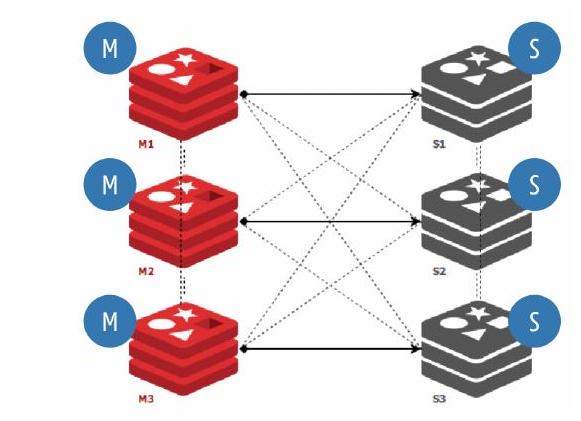
\includegraphics[max width=\textwidth, center]{2024_11_17_21ad14b6196e5740bf69g-6(1)}\\
(a) Redis Cluster (RC) application.\\
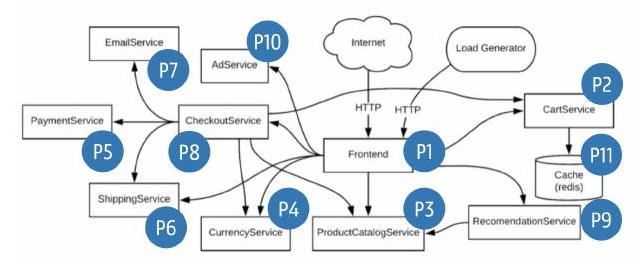
\includegraphics[max width=\textwidth, center]{2024_11_17_21ad14b6196e5740bf69g-6}\\
(b) Online Boutique (OB) application.

Fig. 2: Illustration of microservice dependencies [17], [18].\\
developed for Prometheus has been deployed in the K8s cluster to extract metrics regarding the performance of the RC application. The latency for $\mathrm{RC}\left(\Psi_{a_{1}}\right)$ corresponds to the calculation of the average response time of the Redis server by collecting the total query duration and the total query response time during the last five minutes as shown in (7). The latency threshold $\left(\tau_{a_{1}}\right)$ is set to 250 milliseconds (ms).


\begin{equation*}
\Psi_{a_{1}}=\frac{\text { redis_commands_duration_seconds_total }[5 \mathrm{~m}]}{\text { redis_commands_processed_total }[5 \mathrm{~m}]} \tag{7}
\end{equation*}


The second scenario (Fig. 2b) relates to the OB application [18] consisting of 11 K 8 s deployments. It is a web-based e-commerce application where users can browse items and add them to their cart to purchase them. Recent works have deployed OB to demonstrate novel features in the microservice research domain. The Frontend service receives HTTP\\
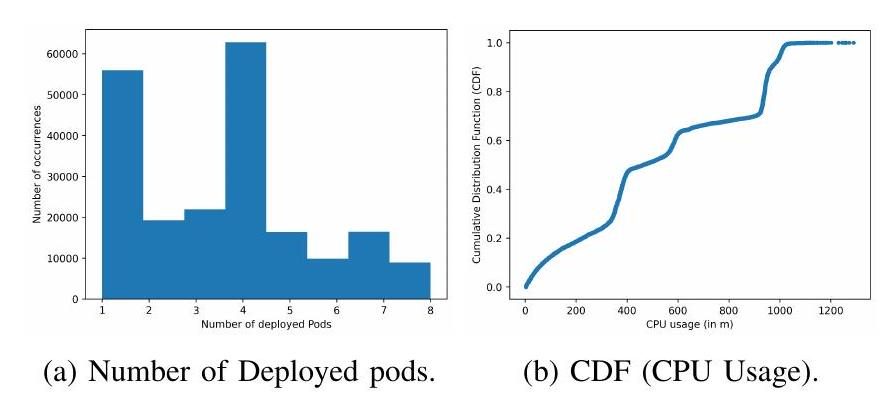
\includegraphics[max width=\textwidth, center]{2024_11_17_21ad14b6196e5740bf69g-7(2)}

Fig. 3: Analysis of the Redis Cluster (RC) master deployment.\\
TABLE VI: Software Versions of the Testbed.

\begin{center}
\begin{tabular}{|l|l|}
\hline
Software & Version \\
\hline
Python \& K8s Python Client & $3.10 \& 23.6 .0$ \\
gym \& stable baselines 3 & $0.21 .0 \& 1.5 .0$ \\
Kubeadm \& Kubectl & v1.22.4 \\
Docker \& Linux Kernel & docker://20.10.10 \& 5.4.0-80-generic \\
Operating System & Ubuntu 20.04.2 LTS \\
\hline
\end{tabular}
\end{center}

TABLE VII: The gym-hpa environment configuration.

\begin{center}
\begin{tabular}{|c|c|c|c|}
\hline
Name & Deploym. & Action Space & Obs. Space \\
\hline
Redis Cluster & 2 & MultiDiscrete(2,15) & 20 states \\
\hline
Online Boutique & 11 & MultiDiscrete(11, 15) & 110 states \\
\hline
\end{tabular}
\end{center}

requests and forwards them to several services, including Currency and Product Catalog. In the evaluation, a load generator based on the locust load tool [47] sends several GET and POST requests from emulated users. The Locust Exporter [48] developed for Prometheus has been deployed in the K8s cluster to collect the average response time of several requests. The latency for $\mathrm{OB}\left(\Psi_{a_{2}}\right)$ corresponds to the average response time based on the GET /cart request as shown in (8). The latency threshold ( $\tau_{a_{2}}$ ) is set to 3 seconds ( 3000 ms ).


\begin{equation*}
\Psi_{a_{2}}=\text { locust_avg_response_time_GET_cart } \tag{8}
\end{equation*}


\section*{B. Dataset creation}
Datasets are collected for both applications from real deployments by generating different requests to trigger several scaling actions. These datasets are saved in Comma Separated Value (CSV) files to help build a tailored simulation where each observation corresponds to the actual resource usage of these applications in a K8s cluster. Fig. 3 shows the number of deployed pods and the corresponding Cumulative Distribution Function (CDF) regarding CPU usage based on the master deployment of the RC application. Based on the selected action by the RL agent, an appropriate observation is retrieved from the dataset, making the simulation mode a near-real experiment.

\section*{C. Testbed implementation}
The gym-hpa framework has been implemented in Python to ease the interaction with both the OpenAI Gym and stable baselines 3 libraries. The K8s Python Client has been used to

TABLE VIII: The execution time per episode during training.

\begin{center}
\begin{tabular}{|c|c|c|c|}
\hline
Algorithm & Application & Mode & Execution Time (in s) \\
\hline
A2C & \multirow{2}{*}{Redis Cluster} & \multirow{2}{*}{Simulation} & $0.445 \pm 0.252$ \\
RPPO &  &  &  \\
\hline
A2C & \multirow{2}{*}{Redis Cluster} & \multirow{2}{*}{Cluster} & $20.090 \pm 6.833$ \\
RPPO &  &  & $24.968 \pm 8.865$ \\
\hline
A2C & \multirow{2}{*}{Online Boutique} & \multirow{2}{*}{Simulation} & $1.262 \pm 0.146$ \\
RPPO &  &  & $1.890 \pm 1.177$ \\
\hline
A2C & \multirow{2}{*}{Online Boutique} & \multirow{2}{*}{Cluster} & $226.30 \pm 58.68$ \\
RPPO &  &  & $285.963 \pm 91.229$ \\
\hline
\end{tabular}
\end{center}

\begin{center}
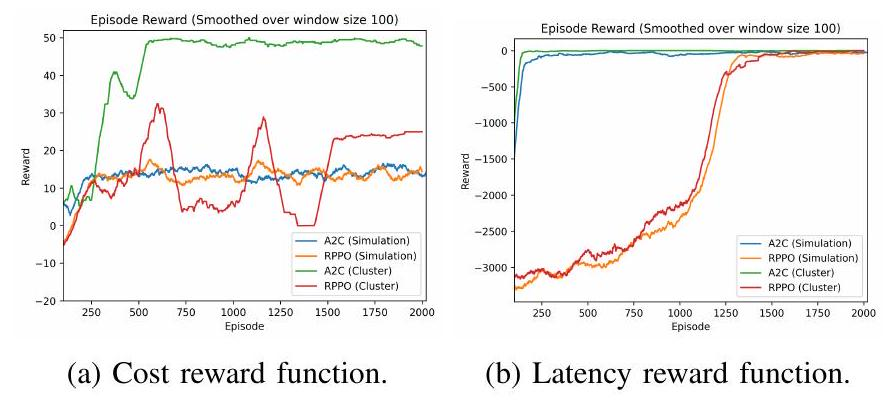
\includegraphics[max width=\textwidth]{2024_11_17_21ad14b6196e5740bf69g-7}
\end{center}

Fig. 4: Accumulated rewards during training for the Redis Cluster (RC) application.\\
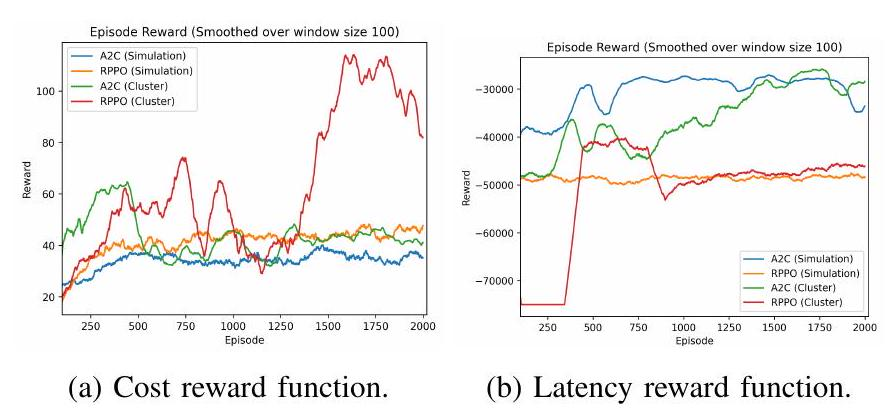
\includegraphics[max width=\textwidth, center]{2024_11_17_21ad14b6196e5740bf69g-7(1)}

Fig. 5: Accumulated rewards during training for the Online Boutique (OB) application.\\
access a K8s cluster and retrieve information from the given deployments. Table VII shows the environment configurations based on the presented applications. In the evaluation, an episode consists of 25 steps where the agent attempts to maximize the reward based on the current demand. Default parameters for both RL agents have been considered, and its optimization is left out of the scope of this paper. The agents have been executed on a 14-core Intel i7-12700H CPU @ 4.7 GHz processor with 16 GB of memory.

\section*{VII. RESUlts}
Table VIII shows the execution time per episode (i.e., 25 steps) during training for both RL algorithms based on the simulation and cluster modes. The simulation mode is significantly faster since the observations come from CSV files rather than retrieved from the K8s API and Prometheus API in the cluster mode. The agents are trained for 2000 episodes, showing that training RL agents in a real cluster is a costly operation. For the RC application, each episode lasts

TABLE IX: Results obtained during the testing phase.

\begin{center}
\begin{tabular}{|c|c|c|c|c|c|}
\hline
\multicolumn{6}{|c|}{Redis Cluster (RC) Application} \\
\hline
Alg. & M & G & Reward & Pods & Latency (in $\mu \mathbf{s}$ ) \\
\hline
A2C & \multirow[t]{2}{*}{S} & \multirow[t]{2}{*}{C} & $24.6 \pm 2.9$ & $2.3 \pm 0.4$ & $55.3 \pm 8.7$ \\
\hline
RPPO &  &  & $26.3 \pm 6.7$ & $2.8 \pm 0.8$ & $107.9 \pm 859.8$ \\
\hline
A2C & \multirow[t]{2}{*}{C} & \multirow[t]{2}{*}{C} & $24.0 \pm 3.2$ & $2.4 \pm 0.6$ & $36.6 \pm 18.2$ \\
\hline
RPPO &  &  & $24.2 \pm 3.0$ & $2.2 \pm 0.3$ & $46.2 \pm 12.1$ \\
\hline
A2C & \multirow[b]{2}{*}{S} & \multirow[t]{2}{*}{L} & -0.4 $\pm 0.1$ & $3.3 \pm 0.9$ & $15.1 \pm 1.5$ \\
\hline
RPPO &  &  & $-0.9 \pm 2.8$ & $3.6 \pm 0.7$ & $23.5 \pm 6.0$ \\
\hline
A2C & \multirow[t]{2}{*}{C} & \multirow[b]{2}{*}{L} & -1.7 $\pm 2.9$ & $13.3 \pm 2.0$ & $28.3 \pm 15.0$ \\
\hline
RPPO &  &  & $-7.0 \pm 36.0$ & $8.4 \pm 4.4$ & $42.4 \pm 11.2$ \\
\hline
KHPA & NA & CPU & NA & $4.1 \pm 0.9$ & $44.8 \pm 34.2$ \\
\hline
\multicolumn{6}{|c|}{Online Boutique (OB) application} \\
\hline
Alg. & M & G & Reward & Pods & Latency (in s) \\
\hline
A2C & \multirow[t]{2}{*}{S} & \multirow[t]{2}{*}{C} & $83.2 \pm 59.7$ & $14.9 \pm 3.0$ & $1.05 \pm 0.48$ \\
\hline
RPPO &  &  & $124.8 \pm 27.2$ & $14.9 \pm 3.1$ & $1.09 \pm 0.27$ \\
\hline
A2C & \multirow[t]{2}{*}{C} & \multirow[t]{2}{*}{C} & $153.6 \pm 32.2$ & $13.1 \pm 3.2$ & $1.28 \pm 0.39$ \\
\hline
RPPO &  &  & $113.7 \pm 41.3$ & $24.8 \pm 8.6$ & $1.17 \pm 0.42$ \\
\hline
A2C & \multirow[t]{2}{*}{S} & \multirow[t]{2}{*}{L} & -25.6K $\pm 3.3 \mathrm{~K}$ & $43.4 \pm 9.6$ & $0.92 \pm 0.16$ \\
\hline
RPPO &  &  & -71.2K $\pm 9.9 \mathrm{~K}$ & $50.7 \pm 6.8$ & $1.08 \pm 0.25$ \\
\hline
A2C & \multirow[b]{2}{*}{C} & \multirow[t]{2}{*}{L} & -34.4K $\pm 6.2 \mathrm{~K}$ & $54.5 \pm 8.6$ & $0.98 \pm 0.52$ \\
\hline
RPPO &  &  & -60.3K $\pm 8.6 \mathrm{~K}$ & $46.3 \pm 6.5$ & $0.99 \pm 0.19$ \\
\hline
KHPA & NA & CPU & NA & $16.7 \pm 3.7$ & $1.22 \pm 0.21$ \\
\hline
\end{tabular}
\end{center}

Mode (M): S = Simulation, C= Cluster, NA = Not Applicable.\\
Goal (G): C = Cost, L = Latency, CPU = CPU usage of $75 \%$.

20 to 25 seconds on average in the cluster mode and takes 0.4 to 0.6 seconds in the simulation mode, with RPPO being slightly slower than A2C. Both algorithms execute slower for the OB application since more microservices are typically deployed. Fig. 4 illustrates the accumulated reward for both reward functions during training for the RC application. The algorithms for the cost function in the cluster mode achieve slightly higher rewards compared to the simulation mode. Regarding the latency function, the algorithms explore the action space to find actions that lead to null rewards since it means that the latency is close to zero. Fig. 5 illustrates the accumulated reward for both reward functions during training for the OB application. A similar pattern occurs compared to the RC application, where the cluster mode achieves higher accumulated rewards than the simulation mode.

In the testing phase, all algorithms have been executed for 100 episodes with the saved configuration after 2000 episodes of training with different demand patterns. Table IX shows the results obtained during the testing phase concerning accumulated rewards, the average number of deployed pods, and the average application latency for the different algorithms for both applications. KHPA has also been evaluated by enabling it for each deployment in the considered applications. Each episode for KHPA consists of the average execution time for each application previously shown in Table VIII, where the number of deployed pods and the application's latency are collected from the K8s cluster. Both algorithms significantly reduce the number of deployed pods or the latency depending on the considered objective for the RC application compared to KHPA. Costs are reduced on average by at least $32 \%$ (e.g., 2.8 versus 4.1 deployed pods), and latency decreased by at least $48 \%$ (e.g., 23.5 versus 44.8 microseconds). The simulation mode achieved lower latency than the cluster mode\\
for latency reduction. In contrast, the cluster mode achieved lower deployment costs than the simulation mode for the cost function, deploying a slightly lower number of pods on average. For the OB application in the cluster mode for the cost objective, A2C reduces costs on average by $20 \%$ compared to KHPA while RPPO increases costs by $30 \%$. Also, for the latency objective, A2C can reduce the expected response time on average by $25 \%$, however, at a high cost in terms of resources since it deploys additional pod instances. A2C outperformed RPPO for the OB application. KHPA cannot find appropriate scaling actions since it does not consider microservice inter-dependencies, and its stabilization window does not allow fast reactions to sudden demands. KHPA only triggers the deployment or termination of pod instances a few seconds after it detects an increase or decrease of demand.

In summary, results show that microservice interdependencies play a major role in the efficient auto-scaling of microservice-based applications. Two distinct objectives have been evaluated, demonstrating that RL algorithms can find appropriate actions by considering microservice interdependencies. In the testing phase, A2C seems more suitable for generalization since it achieved higher rewards than RPPO during different demand patterns. The proposed simulation mode slightly outperformed the cluster mode, demonstrating RL agents can be trained offline with simulations and then validated in operational environments.

\section*{VIII. Conclusions}
This paper presents the gym-hpa framework that bridges the gap between RL and auto-scaling research. The framework is inspired by the OpenAI Gym library and the popular K8s platform, creating a proper environment for RL agents to learn how to perform adequate scaling actions on real cloud environments. The framework has been released in opensource, allowing researchers to evaluate their auto-scaling approaches. In addition, this paper studies microservice interdependencies in auto-scaling since current applications represent complex graphs of loosely-coupled microservices, making its proper scaling a difficult task. The proposed approach aims to improve resource usage and reduce the application's response time in future clouds by applying RL for proper horizontal scaling of microservice applications with complex interdependencies. Experiments showed that RL agents trained with the gym-hpa framework reduce the resource usage on average by at least $30 \%$ and reduce the application's latency by $25 \%$ compared to default auto-scaling mechanisms. As future work, multi-objective RL agents will be studied to find optimal combinations of opposing scaling strategies.

\section*{ACKNOWLEDGMENT}
José Santos is funded by the Research Foundation Flanders (FWO), grant number 1299323N.

\section*{REFERENCES}
[1] N. Dragoni, S. Giallorenzo, A. L. Lafuente, M. Mazzara, F. Montesi, R. Mustafin, and L. Safina, "Microservices: yesterday, today, and tomorrow," Present and ulterior software engineering, pp. 195-216, 2017.\\[0pt]
[2] X. Larrucea, I. Santamaria, R. Colomo-Palacios, and C. Ebert, "Microservices," IEEE Software, vol. 35, no. 3, pp. 96-100, 2018.\\[0pt]
[3] T. Schneider and A. Wolfsmantel, "Achieving cloud scalability with microservices and devops in the connected car domain." in Software Engineering (Workshops), 2016, pp. 138-141.\\[0pt]
[4] Amazon, "Amazon elastic container service (amazon ecs)," accessed on 22 September 2021. [Online]. Available: \href{https://aws.amazon.com/ecs/}{https://aws.amazon.com/ecs/}\\[0pt]
[5] B. Burns, J. Beda, and K. Hightower, Kubernetes: up and running: dive into the future of infrastructure. O'Reilly Media, 2019.\\[0pt]
[6] R. Hat, "Red hat openshift container platform," accessed on 22 September 2021. [Online]. Available: \href{https://www.redhat.com/en/technologies/cloud-computing/openshift}{https://www.redhat.com/en/technologies/cloud-computing/openshift}\\[0pt]
[7] M. Giordani, M. Polese, M. Mezzavilla, S. Rangan, and M. Zorzi, "Toward 6 g networks: Use cases and technologies," IEEE Communications Magazine, vol. 58, no. 3, pp. 55-61, 2020.\\[0pt]
[8] J. Santos, T. Wauters, B. Volckaert, and F. De Turck, "Towards lowlatency service delivery in a continuum of virtual resources: State-of-theart and research directions," IEEE Communications Surveys \& Tutorials, 2021.\\[0pt]
[9] C. Qu, R. N. Calheiros, and R. Buyya, "Auto-scaling web applications in clouds: A taxonomy and survey," ACM Computing Surveys (CSUR), vol. 51, no. 4, pp. 1-33, 2018.\\[0pt]
[10] AWS, "Service auto scaling." accessed on 22 September 2021. [Online]. Available: \href{https://docs.aws.amazon.com/AmazonECS/latest/}{https://docs.aws.amazon.com/AmazonECS/latest/} developerguide/service-auto-scaling.html\\[0pt]
[11] Kubernetes, "Horizontal pod autoscaler." accessed on 22 September 2021. [Online]. Available: \href{https://kubernetes.io/docs/tasks/run-application/horizontal-pod-autoscale/}{https://kubernetes.io/docs/tasks/run-application/horizontal-pod-autoscale/}\\[0pt]
[12] —, "Vertical pod autoscaler," accessed on 22 September 2021. [Online]. Available: \href{https://cloud.google.com/kubernetesengine/docs/concepts/verticalpodautoscaler}{https://cloud.google.com/kubernetesengine/docs/concepts/verticalpodautoscaler}\\[0pt]
[13] Y. Al-Dhuraibi, F. Paraiso, N. Djarallah, and P. Merle, "Autonomic vertical elasticity of docker containers with elasticdocker," in 2017 IEEE 10th international conference on cloud computing (CLOUD). IEEE, 2017, pp. 472-479.\\[0pt]
[14] G. Rattihalli, M. Govindaraju, H. Lu, and D. Tiwari, "Exploring potential for non-disruptive vertical auto scaling and resource estimation in kubernetes," in 2019 IEEE 12th International Conference on Cloud Computing (CLOUD). IEEE, 2019, pp. 33-40.\\[0pt]
[15] G. Brockman, V. Cheung, L. Pettersson, J. Schneider, J. Schulman, J. Tang, and W. Zaremba, "Openai gym," arXiv preprint arXiv:1606.01540, 2016.\\[0pt]
[16] M. Luksa, Kubernetes in action. Simon and Schuster, 2017.\\[0pt]
[17] Redis, "Redis, an open source in-memory data structure store." accessed on 22 September 2021. [Online]. Available: \href{https://redis.io/}{https://redis.io/}\\[0pt]
[18] O. Boutique, "Online boutique, a cloud-native microservices demo application." accessed on 22 September 2021. [Online]. Available: \href{https://github.com/GoogleCloudPlatform/microservices-demo}{https://github.com/GoogleCloudPlatform/microservices-demo}\\[0pt]
[19] I. Gergin, B. Simmons, and M. Litoiu, "A decentralized autonomic architecture for performance control in the cloud," in 2014 IEEE International Conference on Cloud Engineering. IEEE, 2014, pp. 574579.\\[0pt]
[20] A. Danilo, C. Michele, R. Lancellotti, and G. Michele, "A hierarchical receding horizon algorithm for qos-driven control of multi-iaas applications," 2018.\\[0pt]
[21] R. N. Calheiros, E. Masoumi, R. Ranjan, and R. Buyya, "Workload prediction using arima model and its impact on cloud applications' qos," IEEE transactions on cloud computing, vol. 3, no. 4, pp. 449-458, 2014.\\[0pt]
[22] V. R. Messias, J. C. Estrella, R. Ehlers, M. J. Santana, R. C. Santana, and S. Reiff-Marganiec, "Combining time series prediction models using genetic algorithm to autoscaling web applications hosted in the cloud infrastructure," Neural Computing and Applications, vol. 27, no. 8, pp. 2383-2406, 2016.\\[0pt]
[23] J. Kumar and A. K. Singh, "Workload prediction in cloud using artificial neural network and adaptive differential evolution," Future Generation Computer Systems, vol. 81, pp. 41-52, 2018.\\[0pt]
[24] L. Baresi, S. Guinea, A. Leva, and G. Quattrocchi, "A discrete-time feedback controller for containerized cloud applications," in Proceedings of the 2016 24th ACM SIGSOFT International Symposium on Foundations of Software Engineering, 2016, pp. 217-228.\\[0pt]
[25] S. Farokhi, P. Jamshidi, E. B. Lakew, I. Brandic, and E. Elmroth, "A hybrid cloud controller for vertical memory elasticity: A controltheoretic approach," Future Generation Computer Systems, vol. 65, pp. 57-72, 2016.\\[0pt]
[26] S. M. R. Nouri, H. Li, S. Venugopal, W. Guo, M. He, and W. Tian, "Autonomic decentralized elasticity based on a reinforcement learning controller for cloud applications," Future Generation Computer Systems, vol. 94, pp. 765-780, 2019.\\[0pt]
[27] A. N. Toosi, J. Son, Q. Chi, and R. Buyya, "Elasticsfc: Auto-scaling techniques for elastic service function chaining in network functions virtualization-based clouds," Journal of Systems and Software, vol. 152, pp. 108-119, 2019.\\[0pt]
[28] F. Rossi, M. Nardelli, and V. Cardellini, "Horizontal and vertical scaling of container-based applications using reinforcement learning," in 2019 IEEE 12th International Conference on Cloud Computing (CLOUD). IEEE, 2019, pp. 329-338.\\[0pt]
[29] D. Lee, J.-H. Yoo, and J. W.-K. Hong, "Deep q-networks based auto-scaling for service function chaining," in 2020 16th International Conference on Network and Service Management (CNSM). IEEE, 2020, pp. 1-9.\\[0pt]
[30] K. Rzadca, P. Findeisen, J. Swiderski, P. Zych, P. Broniek, J. Kusmierek, P. Nowak, B. Strack, P. Witusowski, S. Hand et al., "Autopilot: workload autoscaling at google," in Proceedings of the Fifteenth European Conference on Computer Systems, 2020, pp. 1-16.\\[0pt]
[31] L. Toka, G. Dobreff, B. Fodor, and B. Sonkoly, "Machine learning-based scaling management for kubernetes edge clusters," IEEE Transactions on Network and Service Management, vol. 18, no. 1, pp. 958-972, 2021.\\[0pt]
[32] P. Singh, P. Gupta, K. Jyoti, and A. Nayyar, "Research on auto-scaling of web applications in cloud: survey, trends and future directions," Scalable Computing: Practice and Experience, vol. 20, no. 2, pp. 399-432, 2019.\\[0pt]
[33] M. Maurer, I. Breskovic, V. C. Emeakaroha, and I. Brandic, "Revealing the mape loop for the autonomic management of cloud infrastructures," in 2011 IEEE symposium on computers and communications (ISCC). IEEE, 2011, pp. 147-152.\\[0pt]
[34] J. Santos, T. Wauters, B. Volckaert, and F. De Turck, "Towards networkaware resource provisioning in kubernetes for fog computing applications," in 2019 IEEE Conference on Network Softwarization (NetSoft). IEEE, 2019, pp. 351-359.\\[0pt]
[35] \_, "Towards delay-aware container-based service function chaining in fog computing," in NOMS 2020-2020 IEEE/IFIP Network Operations and Management Symposium. IEEE, 2020, pp. 1-9.\\[0pt]
[36] Kubernetes, "A deployment provides declarative updates for pods and replicasets." accessed on 28 July 2022. [Online]. Available: \href{https://kubernetes.io/docs/concepts/workloads/controllers/deployment/}{https://kubernetes.io/docs/concepts/workloads/controllers/deployment/}.\\[0pt]
[37] J. Turnbull, Monitoring with Prometheus. Turnbull Press, 2018.\\[0pt]
[38] Kubernetes, "Resource management for pods and containers." accessed on 28 July 2022. [Online]. Available: \href{https://kubernetes.io/docs/concepts/configuration/manage-resourcescontainers/}{https://kubernetes.io/docs/concepts/configuration/manage-resourcescontainers/}.\\[0pt]
[39] V. Medel, R. Tolosana-Calasanz, J. Á. Bañares, U. Arronategui, and O. F. Rana, "Characterising resource management performance in kubernetes," Computers \& Electrical Engineering, vol. 68, pp. 286-297, 2018.\\[0pt]
[40] M. Hessel, J. Modayil, H. Van Hasselt, T. Schaul, G. Ostrovski, W. Dabney, D. Horgan, B. Piot, M. Azar, and D. Silver, "Rainbow: Combining improvements in deep reinforcement learning," in ThirtySecond AAAI Conference on Artificial Intelligence, 2018.\\[0pt]
[41] openAIGym, "The action spaces in openai gym." accessed on 26 July 2022. [Online]. Available: \href{https://github.com/openai/gym/tree/master/gym/spaces}{https://github.com/openai/gym/tree/master/gym/spaces}\\[0pt]
[42] A. Raffin, A. Hill, M. Ernestus, A. Gleave, A. Kanervisto, and N. Dormann, "Stable baselines3," 2019.\\[0pt]
[43] V. Mnih, A. P. Badia, M. Mirza, A. Graves, T. Lillicrap, T. Harley, D. Silver, and K. Kavukcuoglu, "Asynchronous methods for deep reinforcement learning," in International conference on machine learning. PMLR, 2016, pp. 1928-1937.\\[0pt]
[44] D. S. Ratcliffe, K. Hofmann, and S. Devlin, "Win or learn fast proximal policy optimisation," in 2019 IEEE Conference on Games (CoG). IEEE, 2019, pp. 1-4.\\[0pt]
[45] Redis, "How fast is redis?" accessed on 28 August 2022. [Online]. Available: \href{https://redis.io/topics/benchmarks}{https://redis.io/topics/benchmarks}.\\[0pt]
[46] P. Exporter, "Prometheus redis metrics exporter," accessed on 28 August 2022. [Online]. Available: \href{https://github.com/oliver006/redis_exporter}{https://github.com/oliver006/redis\_exporter}.\\[0pt]
[47] Locust, "An open source load testing tool." accessed on 2 December 2021. [Online]. Available: \href{https://locust.io/}{https://locust.io/}.\\[0pt]
[48] C. Solutions, "Locust exporter," accessed on 28 August 2022. [Online]. Available: \href{https://github.com/ContainerSolutions/locust_exporter}{https://github.com/ContainerSolutions/locust\_exporter}.


\end{document}